\chapter{PortAudio}\label{chap:lib}\label{app:portaudio}
As this project requires the usage of the sound card in a computer some interface is needed. A quick search on Google resulted in a countless number of possibilities for interfacing a C++ program with the sound card of a computer. The team decided on a set of requirements which the interface had to provide. The requirements are listed below:

\begin{itemize}
\item Easy-to-use application programming interface.
\item Detailed documentation.
\item Cross platform.
\item Access to raw sample data.
\item Variable sample speed.
\item Support multiple streams (Both recording and playing).
\end{itemize}

% Introduction .. something about why we need a wrapper to the hardware ( Not needed as this is already described in physical layer)
The surface of several interfaces was scratched to see what they had to offer. Some of the best possibilities are listed below:

\begin{description}
\item[RT Audio\footnotemark] was a good option, as it complies with the requirements and is written in C++, but it has a few disadvantages compared to PortAudio. One of the critical points where RT Audio fails, is the documentation. Though it is present, it is not considered good enough compared to what is present in the PortAudio project. It is also worth bringing to notice, that the API is slightly more complicated than PortAudio's.
\footnotetext{\url{http://www.music.mcgill.ca/~gary/rtaudio/}}

\item[QT Multimedia\footnotemark] is developed by Nokia, and is a good suggestion as it complies with the requirements. The disadvantage is that core files from QT itself is needed which results in an increased size of the developed software. It is not that the size is specified as a requirement of the project itself but it also results in a superior complexity of the developed software itself, so QT Multimedia was discarded.
\footnotetext{\url{http://doc.qt.nokia.com/latest/qtmultimedia.html}} 

\item[SDL (Simple Directmedia Layer)\footnotemark]
 is a C library written to provide low-level access to multimedia hardware across platforms, including audio, video, timers and events. It has wrappers to lot of different languages. It has been developed with the main purpose of use in games and demos. The library complies with the requirements, but the extra multimedia functionality is not needed. So this is not an advantage in any way, for which reason PortAudio is a better choice as it has a smaller footprint.
\footnotetext{\url{http://www.libsdl.org/}}

\item[CLAM\footnotemark] is short for C++ Library for Audio and Music, and provides lot of communication possibilities with the sound hardware. This library supports both low and high level interface with the hardware as well as built in support for FFT. After further investigations on this library, it turned out that the documentation was very poor, and therefore it was discarded as a possible sound interface.
\footnotetext{\url{http://clam-project.org}}

\item[PortAudio\footnotemark] was finally chosen as the lowermost component of the software as it complies with the requirements mentioned above.  The reason for this final decision was based on the simplicity of the usage of PortAudio. Furthermore it is extremely adaptable which makes it possible to use in a wide range of applications. A block diagram showing the supported sound platforms can be seen in Figure \ref{fig:app_portaudio}.
\footnotetext{\url{http://www.portaudio.com/}}
\end{description}

\begin{figure}[htb]
	\begin{center}
	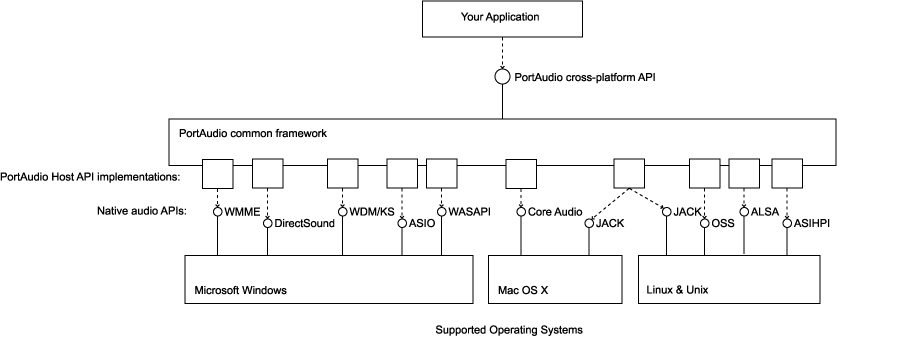
\includegraphics[scale=0.44,trim=0 0 0 0]{content/graphics/appendix/portaudio_architecture.png}%trim=l b r t
	\caption{This is an overview of the PortAudio interface.}
	\label{fig:app_portaudio}
	\end{center}
\end{figure}
